% The exercise requires:
% The solutions require:

\begin{samproblem}*{}{Arrow matrix-vector multiplication}[1](1){
    An ``arrow matricx'' $\VA$ is constructed given two vectors $\mathbb{a}$ and $\mathbb{d}$.
    The matrix is then squared and multiplied with a vector $\Vx$. This is implemented in the
    following C++ function:

\samincludecpp{./PROBLEMS/Codes/MatVec/arrowmatvec.cpp}

}

%%%%%%%%%%%% SUBPROBLEM 1
\begin{subproblem}{}

  For general vectors $\mathbb{d} = (d_1, \dots, d_n)^\top$ and $\mathbb{a} = (a_1, \dots, a_n)^\top$
  sketch the matrix $\VA$ created in the function \verb|ArrowMatrixSquaredTimes|.

  \begin{samwriteprbpart}{sol}
  \begin{samsolution}
    The matrix $\mathbb{A}$ is the following:
    \begin{align}
    \VA=\begin{pmatrix}
      d_1 &     &        &         & a_1     \\
          & d_2 &        &         & a_2     \\
          &     & \ddots &         & \vdots  \\
          &     &        & d_{n-1} & a_{n-1} \\
      a_1 & a_2 & \dots  & a_{n-1} & d_n     \\
    \end{pmatrix}
    \end{align}
    The file \texttt{???} contains a detailed description of the code.
  \end{samsolution}
\end{samwriteprbpart}
\end{subproblem}

%%%%%%%%%%%% SUBPROBLEM 2
\begin{subproblem}
  We measure the run time of the function \texttt{} (in file \texttt{arrowmatvec.cpp})
  and plot the results in Figure \ref{fig:arrowmatvectiming}.

  Give a detailed explanation of the results.

% \begin{figure}[ht]
% \centering
% 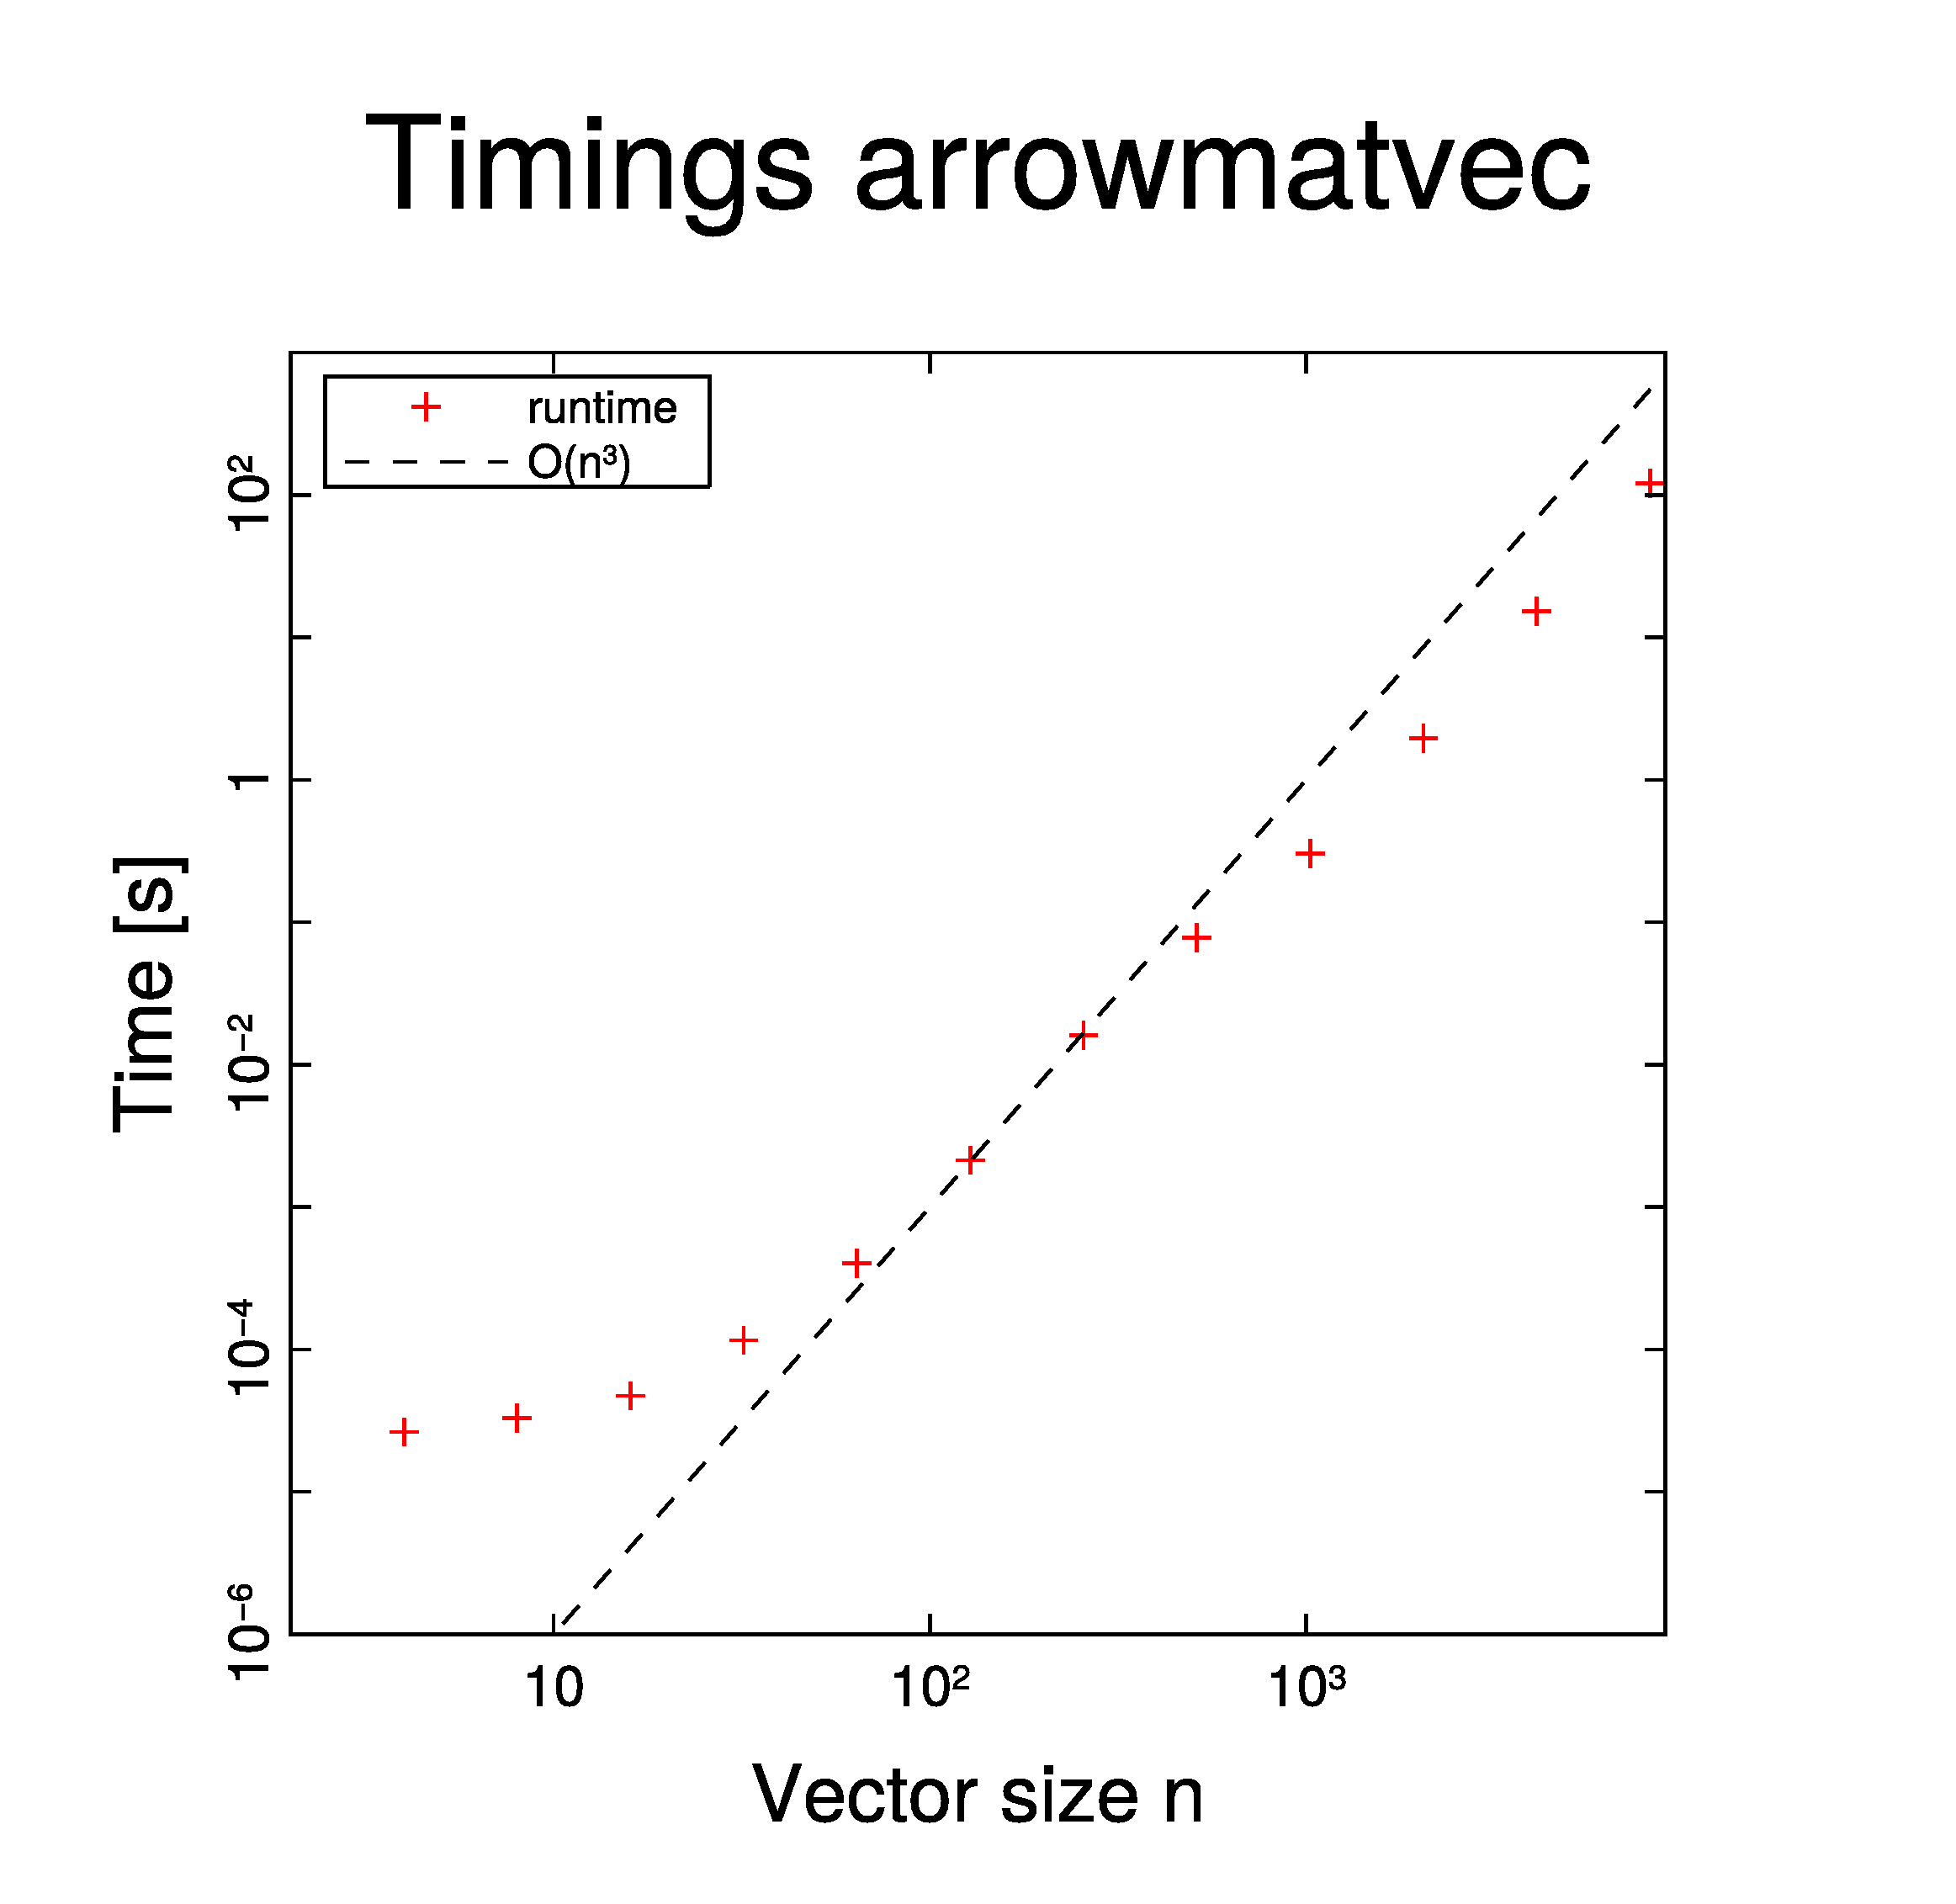
\includegraphics[width=0.8\textwidth]{\problems/\chpt/PICTURES/arrowmatvectiming.eps}
% \caption{timings for \texttt{arrowmatvec(d,a,x)}}
% \label{fig:arrowmatvectiming}
% \end{figure}

 \begin{samwriteprbpart}{sol}
\begin{samsolution}
  The standard matrix-matrix multiplication has runtime growing with $O(n^3)$ and the standard
  matrix-vector multiplication has runtimes growing with $O(n^2)$. Hence, the overall
  computational complexity is dominated by $O(n^3)$.

  Remember that most of C++ operators have a \textbf{left-to-right} precedence. This means that,
  even if,
  mathematically, $(\mathbf{A} \mathbf{A}) \mathbf{y} = \mathbf{A} (\mathbf{A} \mathbf{y})$, when
  implementing the expression in C++, the \emph{complexity} of the code will be very different.

  Remark: even Eigen's own internal template expression mechanism is not able to efficiently
  exploit this fact.
\end{samsolution}
\end{samwriteprbpart}
\end{subproblem}

%%%%%%%%%%%% SUBPROBLEM 3
\begin{subproblem}
Write an \emph{efficient} C++ function
\begin{verbatim}
  void efficient_arrow_matrix_2_times_x(const VectorXd & d, const VectorXd & a,
                              const VectorXd & x, VectorXd & y)
\end{verbatim}
that computes the same multiplication as in code \ref{mc:ArrowMatrixVector_arrowmatvec} but
with optimal asymptotic complexity with respect to {$n$}. Compute the complexity of your code and explain why you obtain the result.
Here \texttt{d} passes the vector $(d_{1},\ldots,d_{n})^{T}$ and \texttt{a} passes the
vector $(a_{1},\ldots,a_{n})^{T}$.
 \begin{samwriteprbpart}{sol}
\begin{samsolution}
  Due to the special structure of the matrix, it is possible to write a more efficient
  implementation than the standard matrix-vector multiplication.

  We can rewrite $\mathbf{A}$ as follows:


  See code listing \ref{mc:ArrowMatrixVector_arrowmatvec2}.
\vspace{0.5cm}

% \lstinputlisting[caption={implementation of the function \texttt{arrowmatvec2}},label={mc:ArrowMatrixVector_arrowmatvec2}]
% {\problems/\chpt/MATLAB/arrowmatvec2.m}
\end{samsolution}
\end{samwriteprbpart}
\end{subproblem}

%%%%%%%%%%%% SUBPROBLEM 4
\begin{subproblem}
What is the complexity of your algorithm from sub-problem
\ref{subprb:ArrowMatrixVector_3} (with respect to samproblem size $n$)?
 \begin{samwriteprbpart}{sol}
\begin{samsolution}
  The efficient implementation only needs two vector-vector element-wise multiplications and
  one vector-scalar multiplication. Therefore the complexity is $O(n)$.
\end{samsolution}
\end{samwriteprbpart}
\end{subproblem}

%%%%%%%%%%%% SUBPROBLEM 5

\begin{subproblem}
  Compare the runtime of your implementation and the implementation given in code
  \ref{mc:ArrowMatrixVector_arrowmatvec} for $n=2^{5,6,\ldots,12}$.
  Use the routines as explained in example
  \ref{ex:effmatmult} of the Lecture Slides.
 \begin{samwriteprbpart}{sol}
\begin{samsolution}
The standard matrix multiplication has runtimes growing with $O(n^3)$.
The runtimes of the more efficient implementation are growing with $O(n)$.
See \autoref{mc:ArrowMatrixVector_arrowmatvec2timing} and Figure~\ref{fig:arrowmatvec2timing}.

% \lstinputlisting[caption={Execution and timings of \texttt{arrowmatvec} and \texttt{arrowmatvec2}}, label={mc:ArrowMatrixVector_arrowmatvec2timing}]
% {\problems/\chpt/MATLAB/arrowmatvec2timing.m}

% \begin{figure}[ht]
% \centering
% 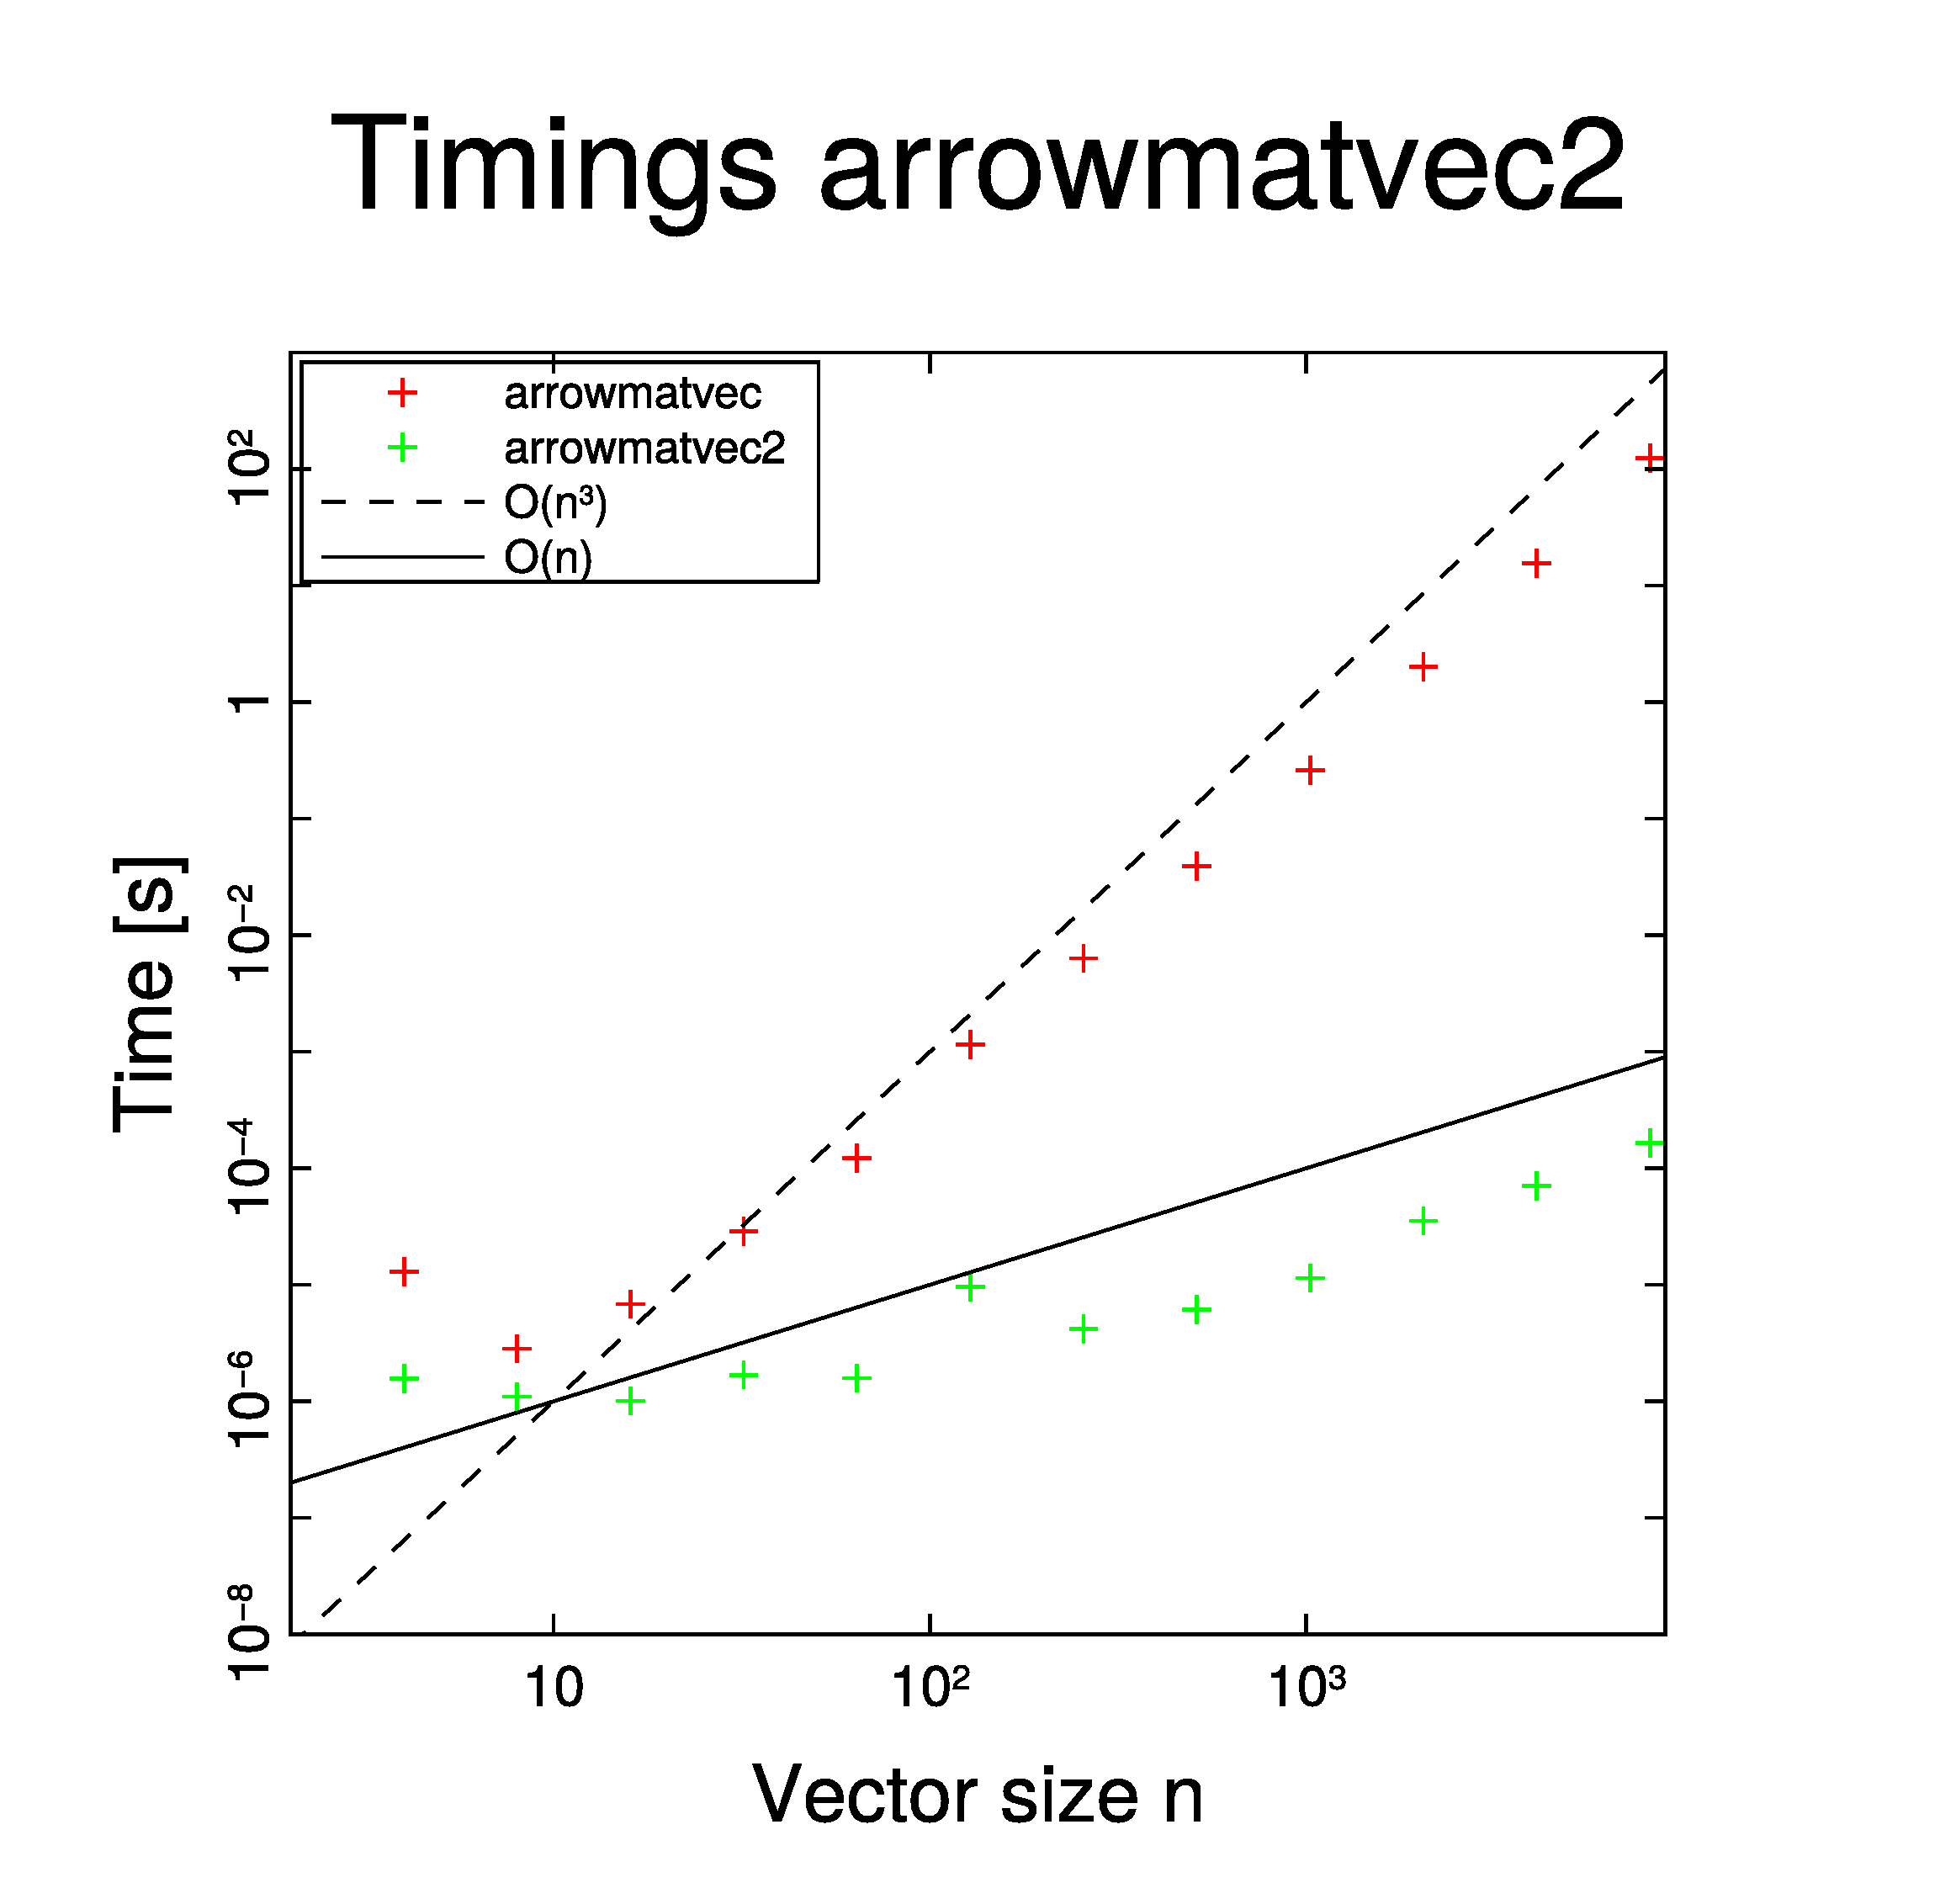
\includegraphics[width=0.8\textwidth]{\problems/\chpt/PICTURES/arrowmatvec2timing.eps}
% \caption{timings for \texttt{arrowmatvec2(d,a,x)}} \label{fig:arrowmatvec2timing}
% \end{figure}
\end{samsolution}
\end{samwriteprbpart}
\end{subproblem}

\end{samproblem}
